\chapter*{List of Publications}
\addcontentsline{toc}{chapter}{List of Publications}
\setheader{List of Publications}
\label{publications}

%% We use the 'etaremune' environment (the reverse of 'enumerate') to get a
%% numbered list of publications in reverse chronological order. If the list of
%% authors is long, it might be useful to emphasize your own name with \textbf.
\begin{enumerate}{\small
\item {M.\ Piro}, {M.\ Poschmann} and \textbf{P.\ Bajpai}, \textit{On the interpretation of chemical potentials computed from equilibrium thermodynamic codes: Applications to molten salts}, \href{https://doi.org/10.1016/j.jnucmat.2019.151756}{Journal of Nuclear Materials, 526 (2019) 151756}.
\item \textbf{P.\ Bajpai}, {M.\ Poschmann}, {M.\ Piro}, \textit{Derivations of useful partial molar excess Gibbs energy of mixing expressions of common thermodynamic models}, To be submitted to \href{https://www.journals.elsevier.com/calphad}{CALPHAD Computer Coupling of Phase Diagrams and Thermochemistry}. [In preparation]
\item \textbf{P.\ Bajpai}, {M.\ Poschmann}, {D.\ Andr\v{s}}, {C.\ Bhave}, {M.\ Tonks} and {M.\ Piro}, \textit{Development of a new thermochemistry solver for multiphysics simulations of nuclear materials}, \href{http://https://www.tms.org/TMS2020}{TMS 2020 Supplemental Proceedings, TMS 2020  - 149\textsuperscript{th} Annual Meeting \& Exhibition, San Diego, February 23-27, 2020}. [Accepted]
\item \textbf{P.\ Bajpai}, {M.\ Poschmann}, {D.\ Andr\v{s}} and {M.\ Piro}, \textit{Progress in developing a new thermochemistry code for corrosion modelling and multiphysics simulation of nuclear fuels}, \href{http://cns-annual-conference.org/2019/index.html}{39\textsuperscript{th} Annual Conference of the Canadian Nuclear Society and 43\textsuperscript{rd} Annual CNS/CNA Student Conference, Ottawa, June 23-26, 2019}.
}\end{enumerate}

\setboolean{@twoside}{false}

\newpage
\dedication{{M.\ Piro}, {M.\ Poschmann} and \textbf{P.\ Bajpai} \\ \textit{On the interpretation of chemical potentials computed from equilibrium thermodynamic codes: Applications to molten salts}\\ \href{https://doi.org/10.1016/j.jnucmat.2019.151756}{Journal of Nuclear Materials, 526 (2019) 151756}.}

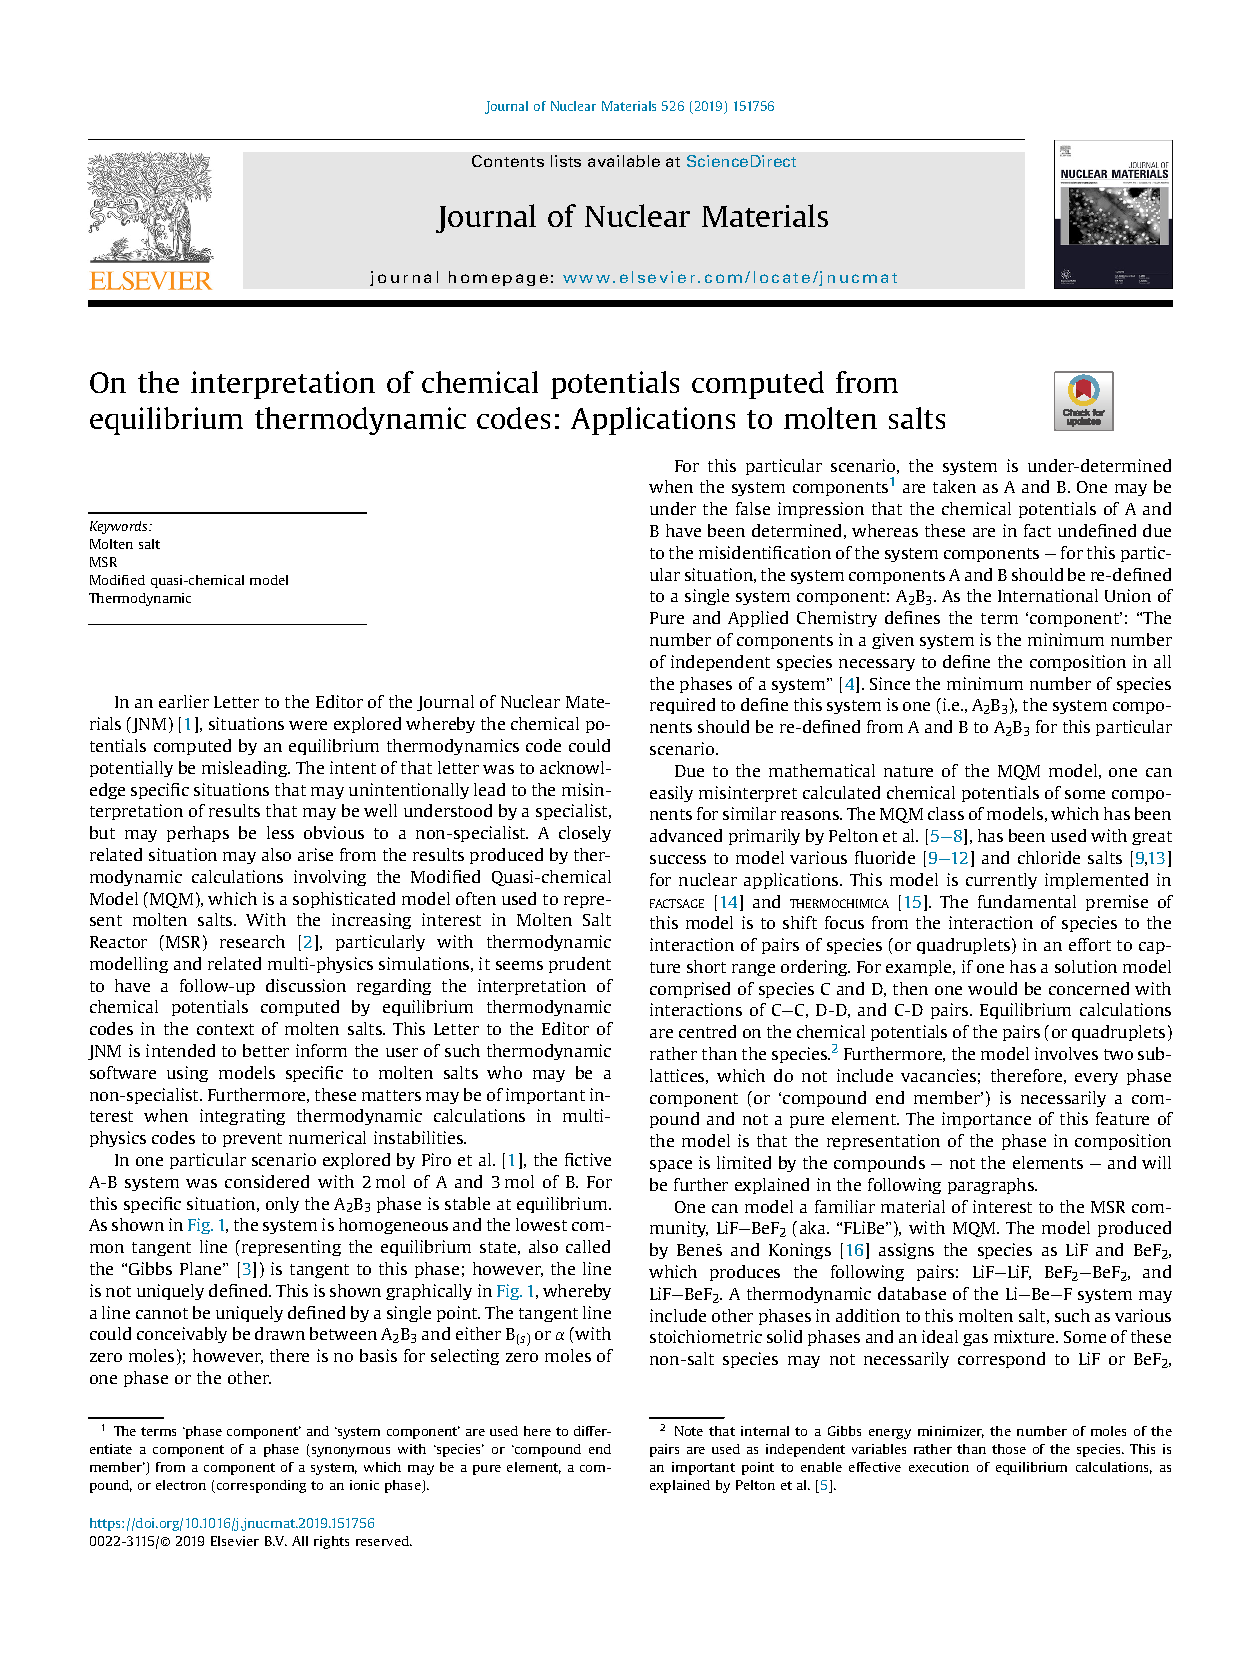
\includepdf[pages=-]{publications/Piro_JNM_2019.pdf}

\newpage
\dedication{\textbf{P.\ Bajpai}, {M.\ Poschmann} and {M.\ Piro}\\ \textit{erivations of useful partial molar excess Gibbs energy of mixing expressions of common thermodynamic models}\\ To be submitted to \href{https://www.journals.elsevier.com/calphad}{CALPHAD Computer Coupling of Phase Diagrams and Thermochemistry}. [In preparation]}

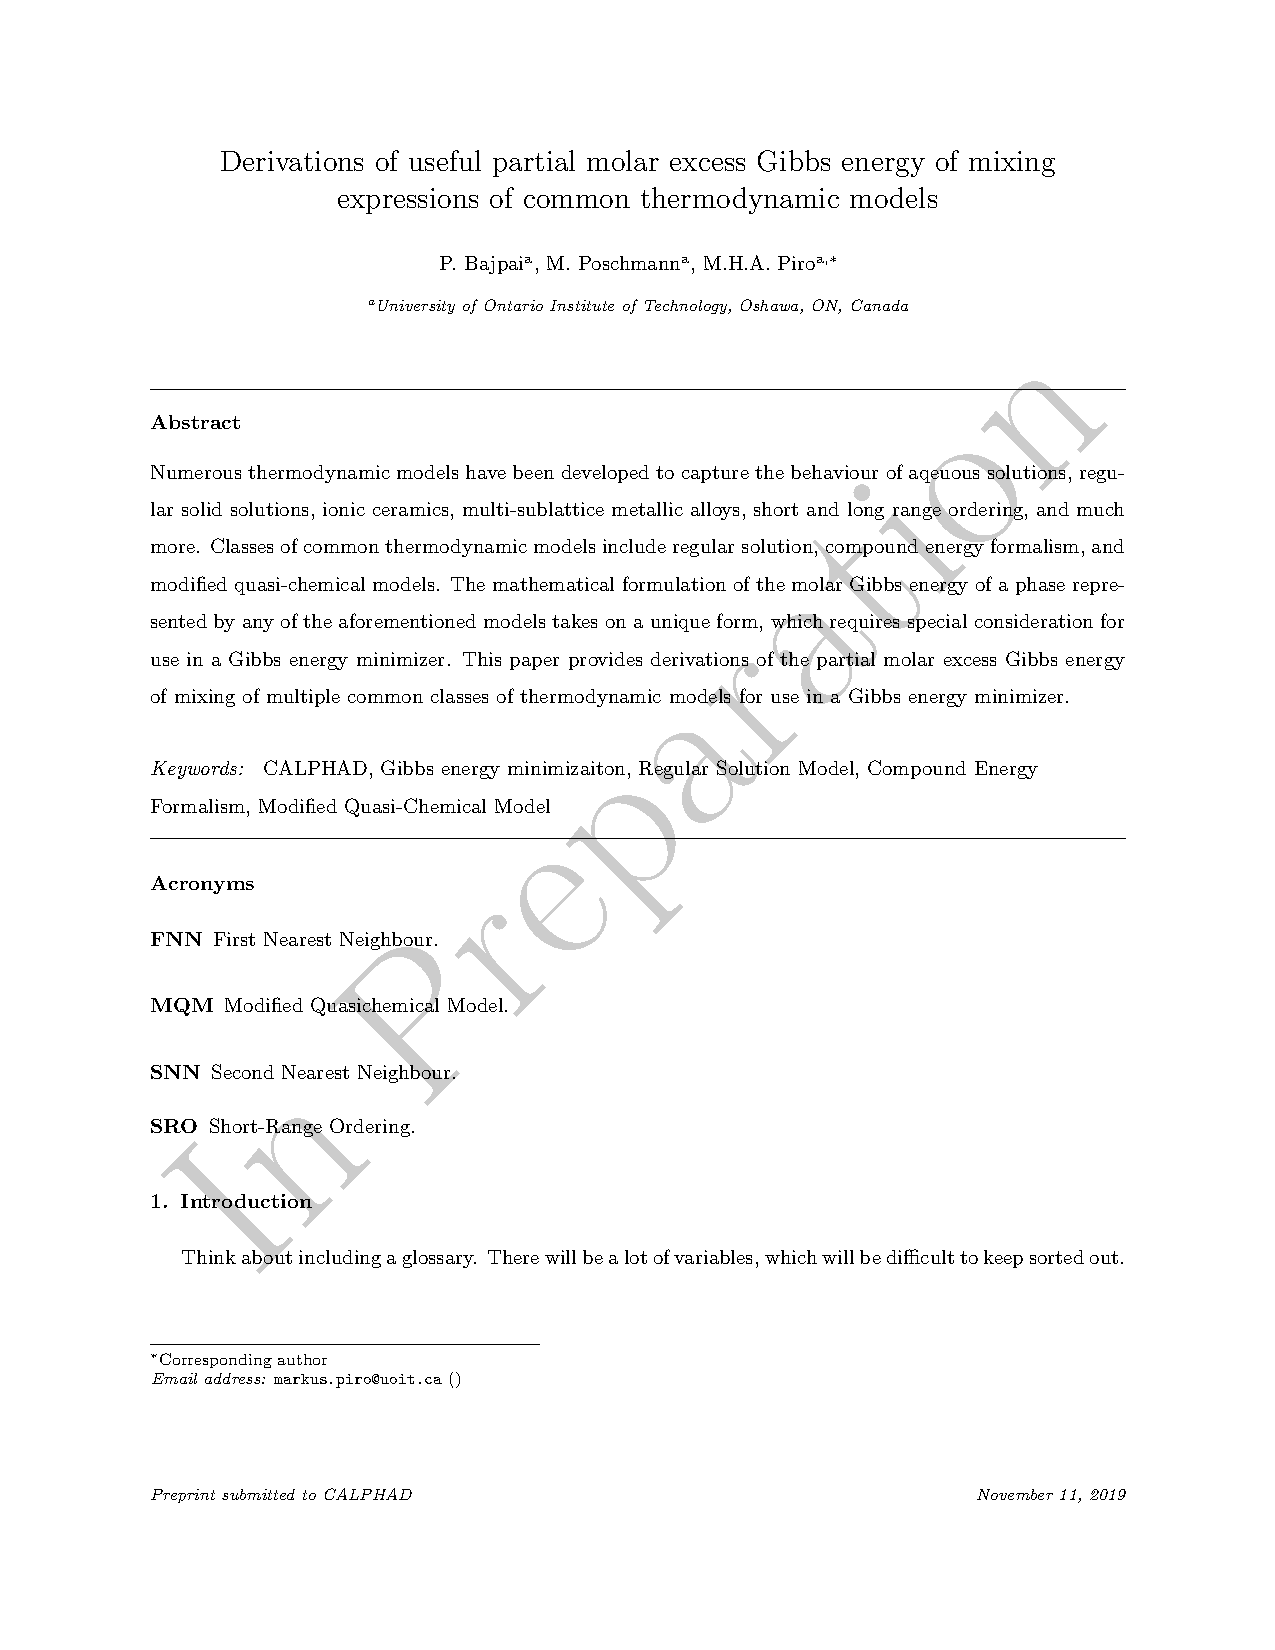
\includepdf[pages=-]{publications/Bajpai_Calphad_2020.pdf}

\newpage
\dedication{\textbf{P.\ Bajpai}, {M.\ Poschmann}, {D.\ Andr\v{s}}, {C.\ Bhave}, {M.\ Tonks} and {M.\ Piro}\\ \textit{Development of a new thermochemistry solver for multiphysics simulations of nuclear materials}\\ \href{http://https://www.tms.org/TMS2020}{TMS 2020 Supplemental Proceedings, TMS 2020  - 149\textsuperscript{th} Annual Meeting \& Exhibition, San Diego, February 23-27, 2020}. [Accepted]}
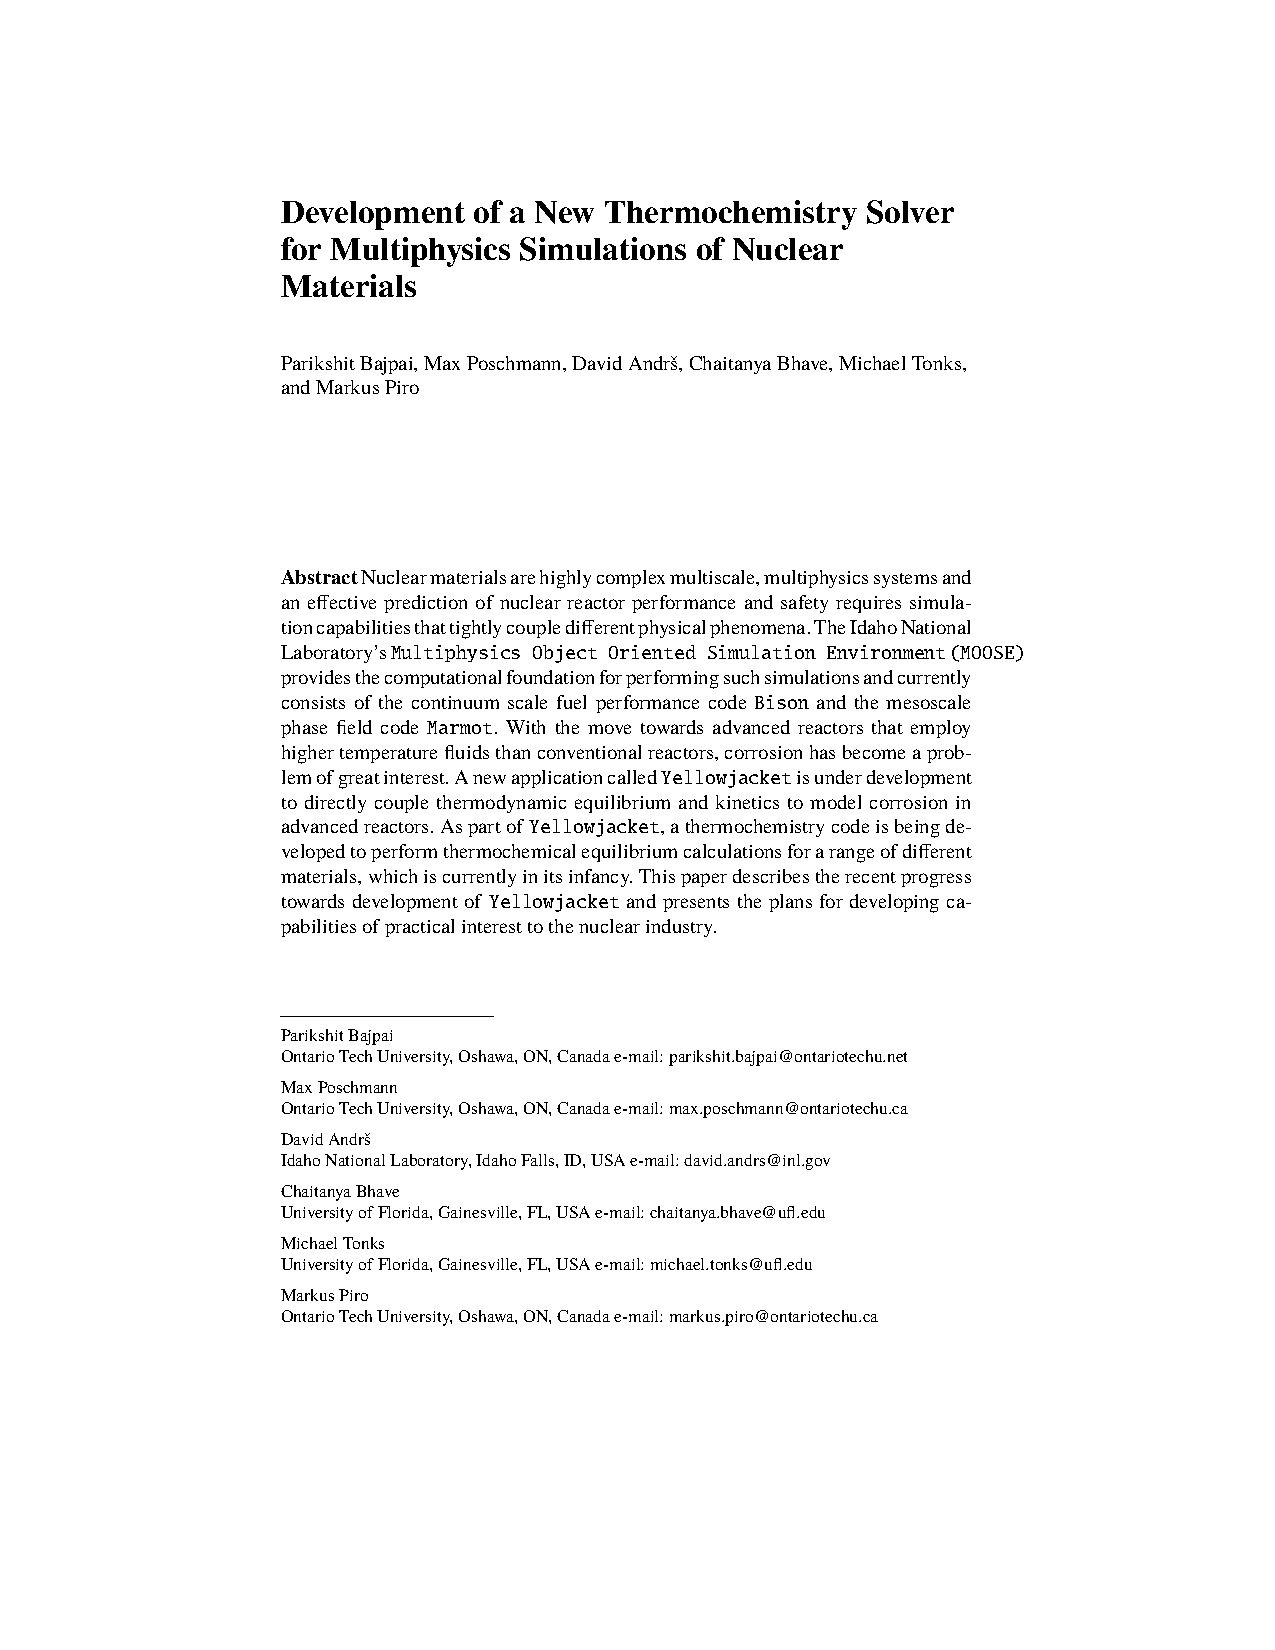
\includepdf[pages=-]{publications/Bajpai_TMS_2020.pdf}


\setboolean{@twoside}{false}

\newpage
\dedication{
\textbf{P.\ Bajpai}, {M.\ Poschmann}, {D.\ Andr\v{s}} and {M.\ Piro}\\ \textit{Progress in developing a new thermochemistry code for corrosion modelling and multiphysics simulation of nuclear fuels}\\ \href{http://cns-annual-conference.org/2019/index.html}{39\textsuperscript{th} Annual Conference of the Canadian Nuclear Society and 43\textsuperscript{rd} Annual CNS/CNA Student Conference, Ottawa, June 23-26, 2019}.}
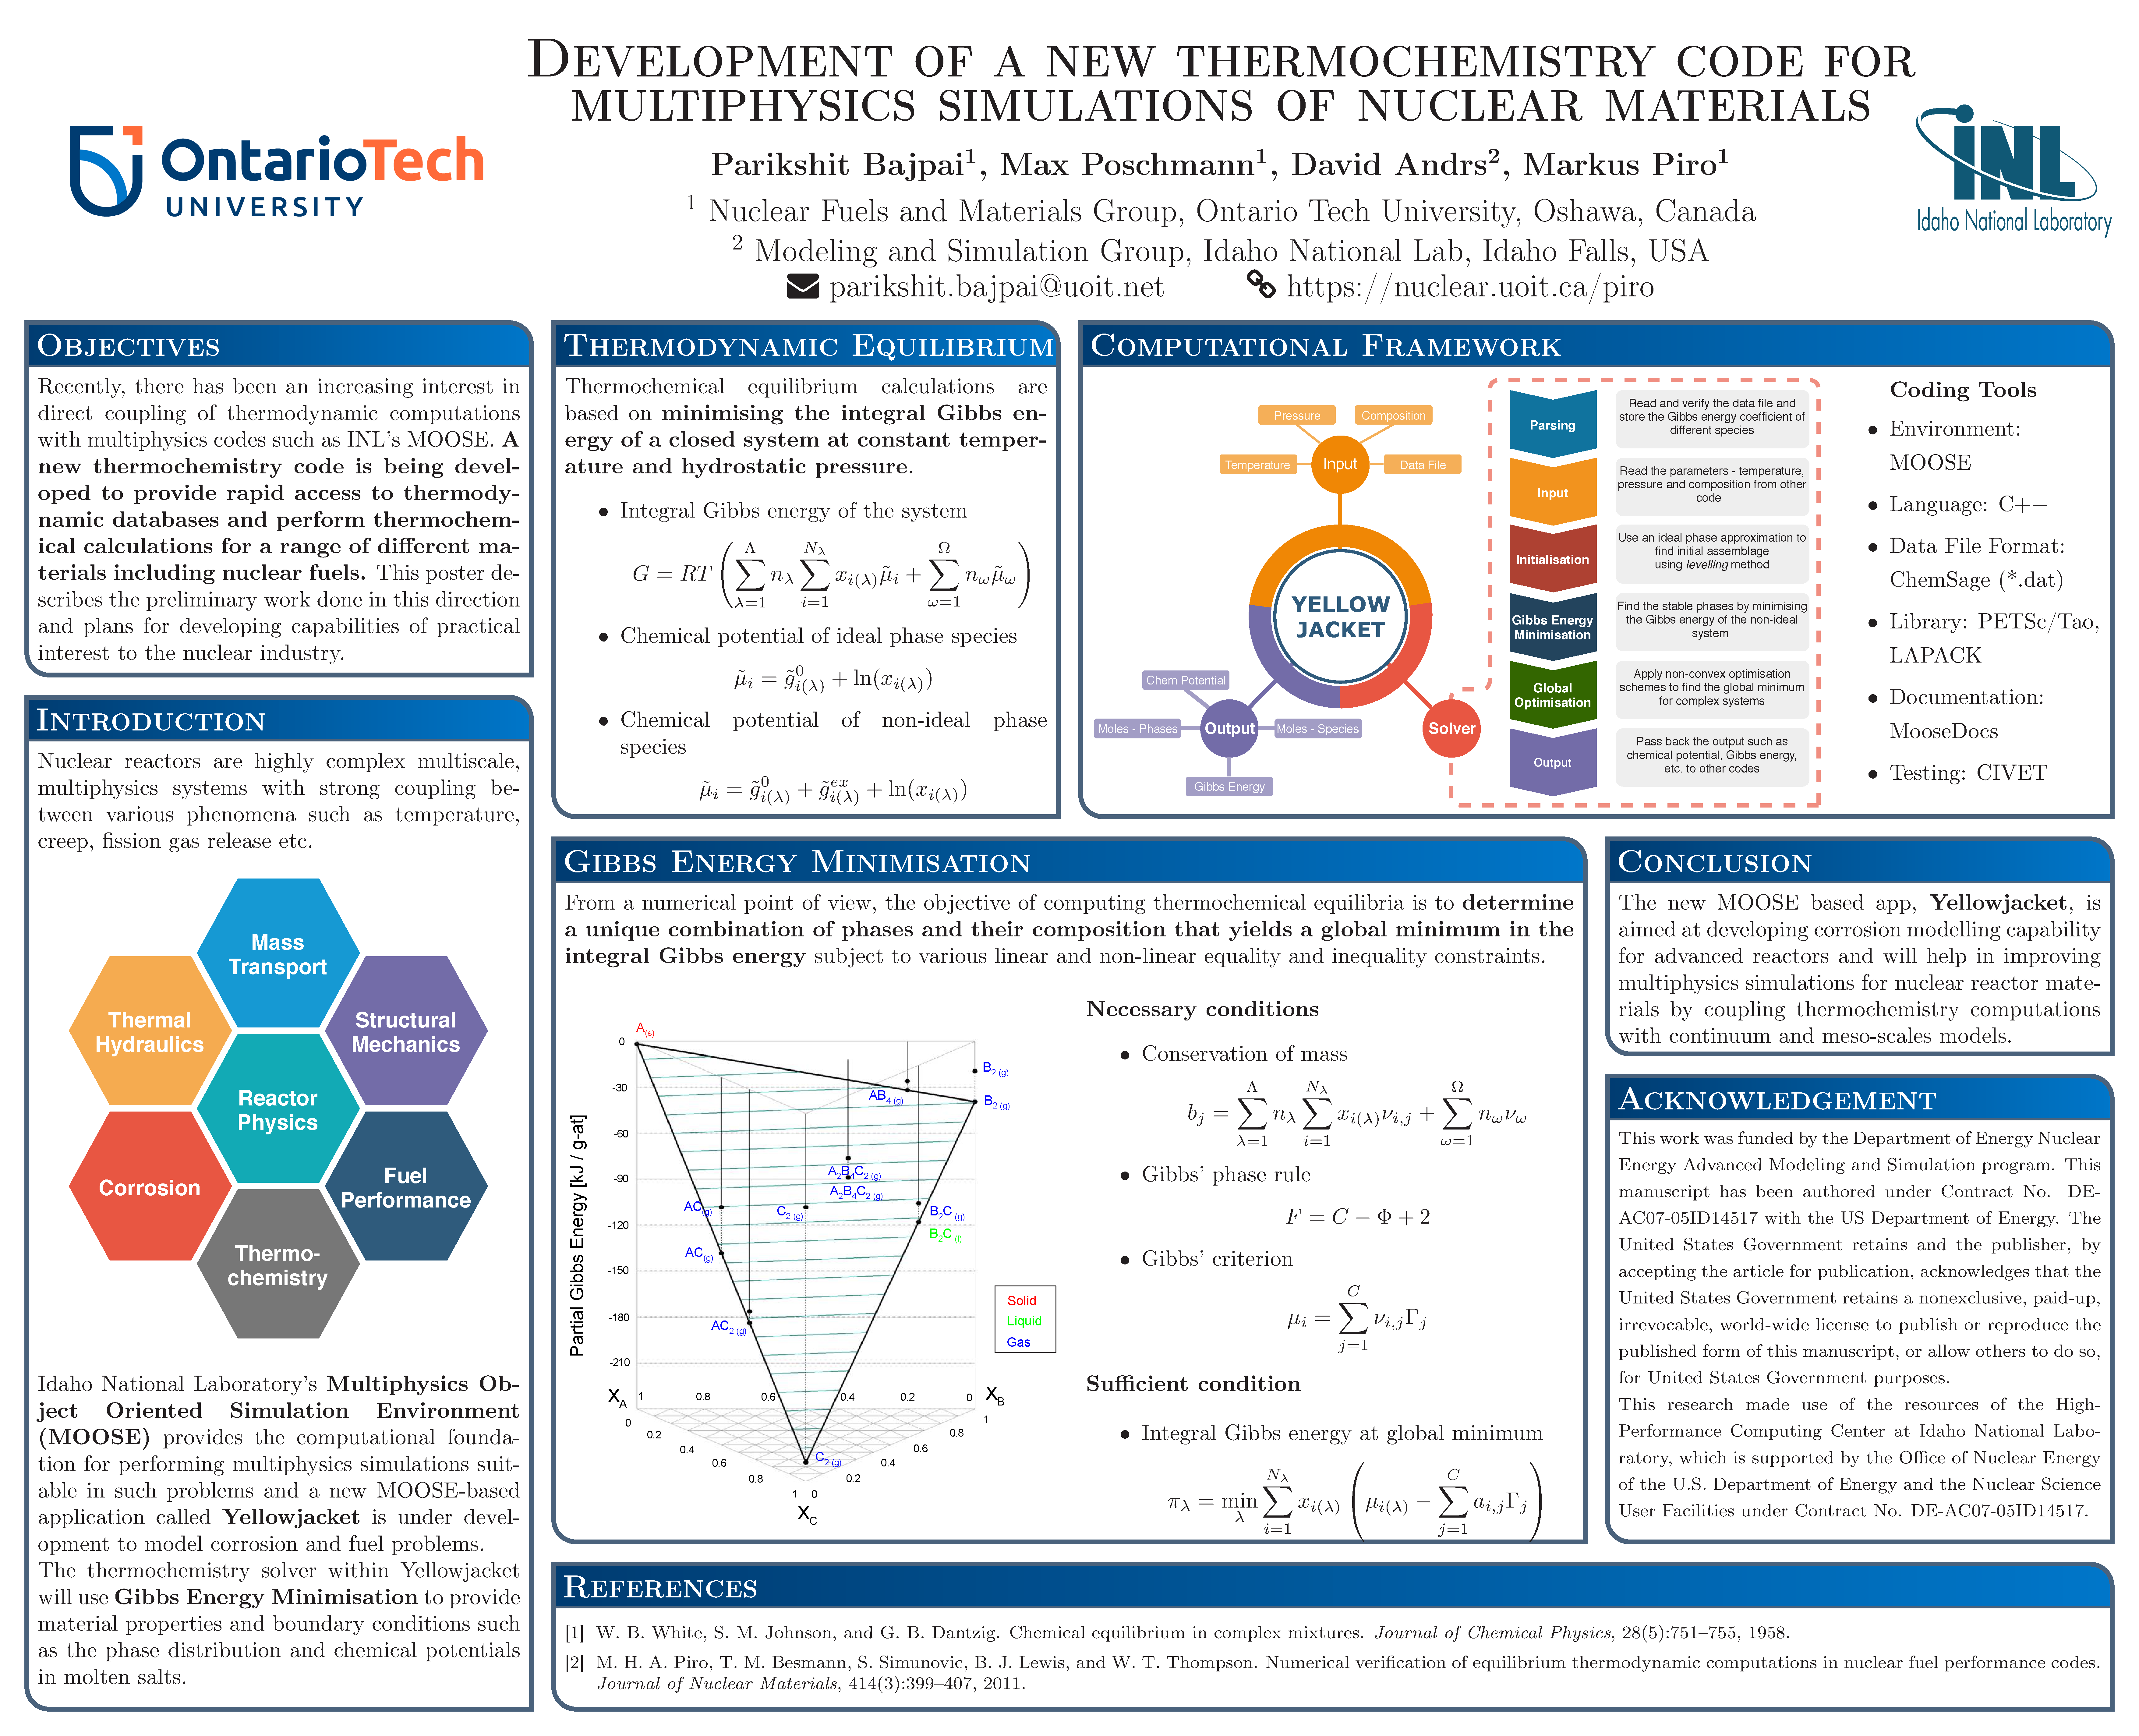
\includepdf[pages=-]{publications/CNS_Poster.pdf}
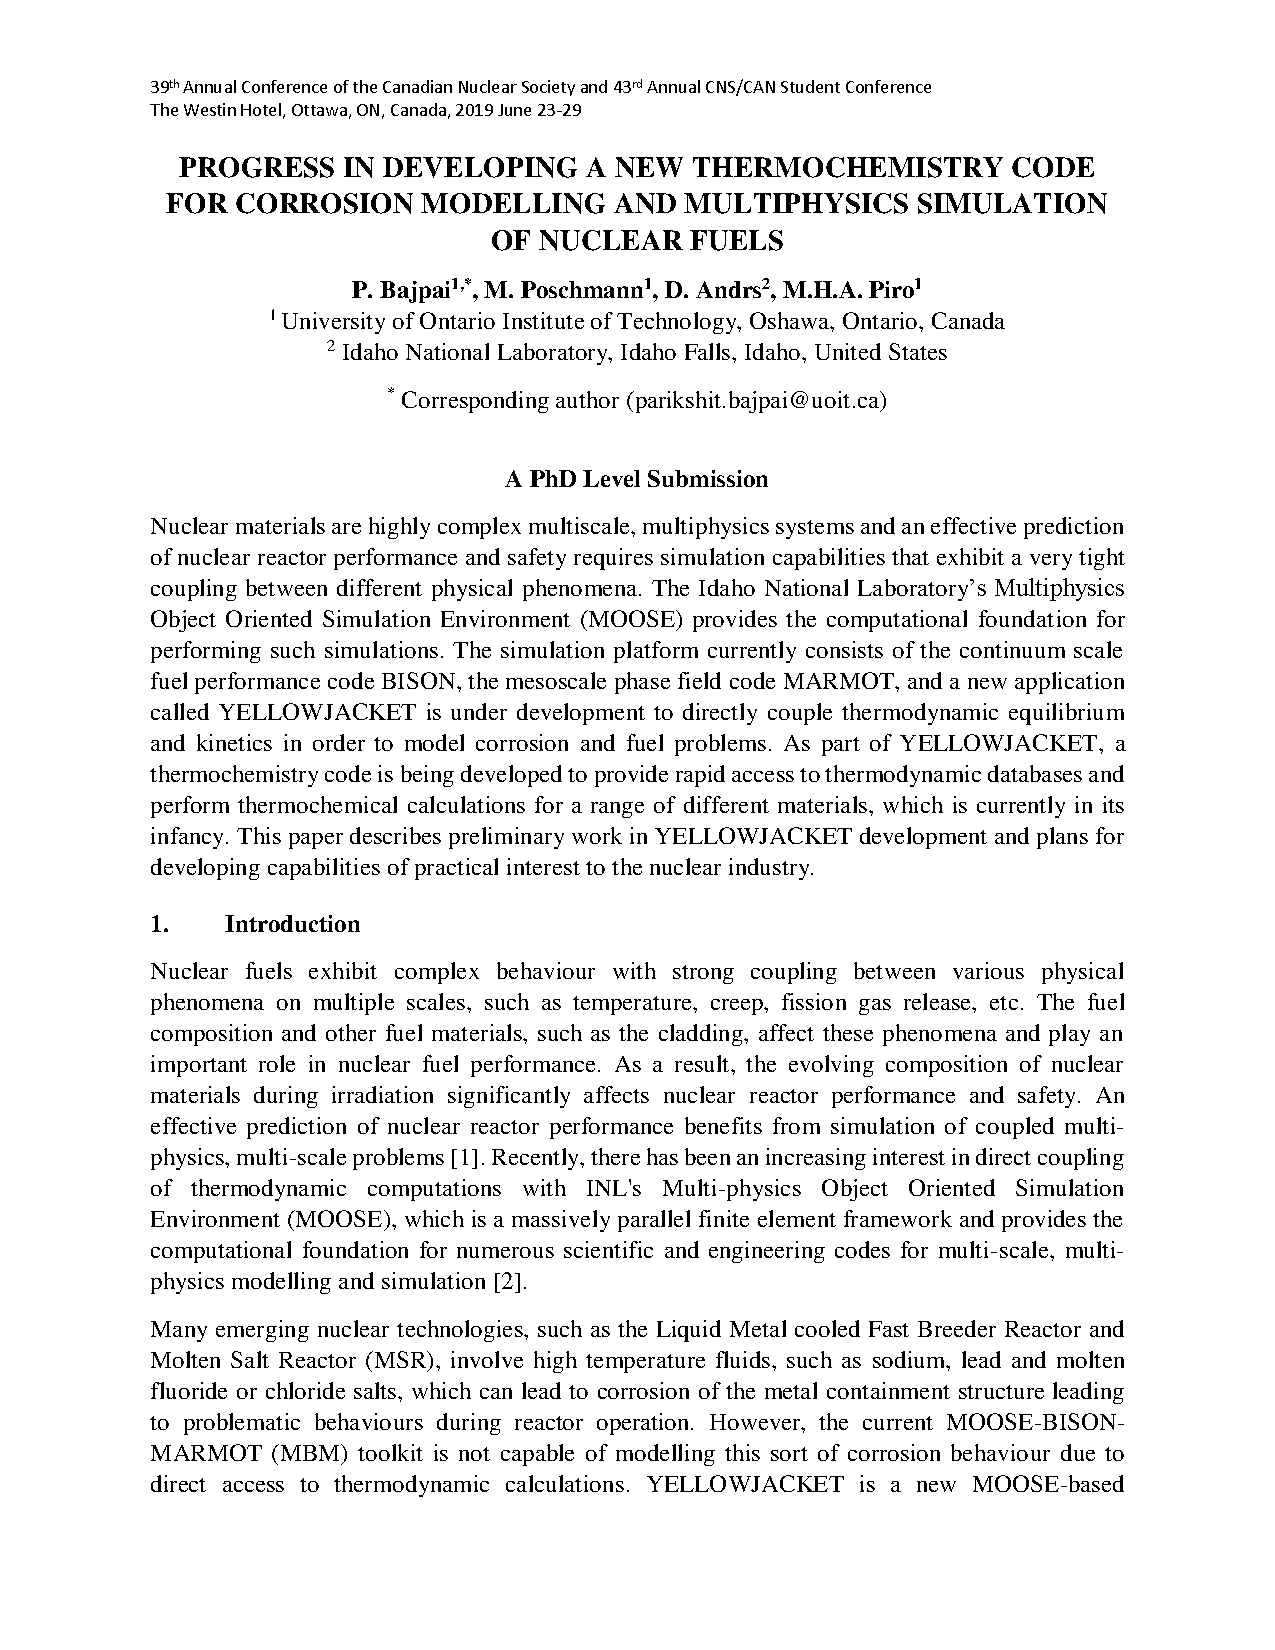
\includepdf[pages=-]{publications/Bajpai_CNS_2019.pdf}

\setboolean{@twoside}{false}
